\documentclass[12pt, a4paper]{article}
% \usepackage{mathtools}
\usepackage{graphicx}
\usepackage{amsthm}
\usepackage{hyperref}
\usepackage{amssymb}
\graphicspath{{images/}}

\hypersetup{
    colorlinks=true,
    linkcolor=blue,
    urlcolor=cyan
}

\title{AP Stats Notes}
\author{Franklin Chen}
\date{11 November 2024 - idk some time in may}

\theoremstyle{definition}
\newtheorem{definition}{Definition}

\begin{document}
\maketitle
\newpage
% comment

\tableofcontents
\newpage

using \textit{The Practice of Statistics for the AP Exam: 6th Edition} by Starnes and Tabor

\section{Data Analysis}
\subsection{What is Statistics?}

\begin{definition}[Statistics]
    The science of collecting, analyzing, and drawing conclusions from data.
\end{definition}

Data is collected from \emph{individuals} about certain \emph{variables}.

\begin{definition}[Individual, Variable]
    
    \textbf{Individuals} are objects described in a dataset. Typically people, but not always.
    
    \textbf{Variables} are attributes that can take different values for different individuals.
\end{definition}

For example, \emph{individuals} may be households, and \emph{variables} may be region, nnumber of people, household income, etc. It's important to distinguish between \emph{categorial} and \emph{quantative} variables:

\begin{definition}[Categorical and Quantative Variables]
    \textbf{Categorical Variables} are variables whose values can be placed into distinct categories.

    \textbf{Quantative Variables} are variables whose values are quantities, typically counts or measurements.
\end{definition}

For example, region would be categorical, while household income would be quantative. \emph{Not all numbers are quantative}; eg. zip code.

\subsection{Analyzing Categorical Data}
\subsubsection{One-Variable Categorical Data}
\begin{definition}[Frequency and Relative Frequency Tables]
    \textbf{Frequency Tables}shows the number of individuals that have values of a certain category. \textbf{Relative Frequency Tables} shows the proportion or percent of individuals in each category.
\end{definition}

\emph{Note (relative) frequencies are not data; they \emph{summarize} data.} Bar graphs and Pie Graphs summarize relative frequency tables.

\emph{Beware of misleading graphs}; we mainly react to the area of each bar, not the actual height.

\subsubsection{Two-Variable Categorical Data}
Use a two-way table to summarize data about two categorical variables. These tables can be used to answer questions about \emph{marginal, joint, and conditional relative frequencies.}
\begin{figure}[t]
    \centering
    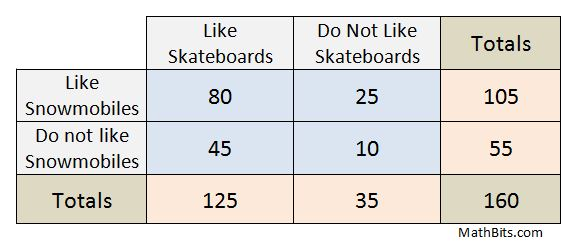
\includegraphics[width=0.75\textwidth]{two way table.png}
    \caption{An example two-way table with additional summary information.}
    \label{fig:two-way-table}
\end{figure}

\textbf{Margial relative frequencies} give the percent or proportion of individuals that have a given value for one categorical variable. For example, the marginal relative frequency of liking skateboards is $\frac{125}{160} \approx 78.125\%$.

\textbf{Joint relative frequencies} give the percent or proportion of individuals that have a specific value for both categorical variables. For example, the joint frequency of liking both skateboards and snowmobiles is $\frac{80}{160} = 50\%$.

\textbf{Conditional relative frequencies} give the percent or proportion of individuals that have a specific value for one categorical variable relative to other individuals with the same other categorical variable. For example, the conditional relative frequency of those who like snowmobiles out of all individuals that like skateboards is $\frac{80}{125} = 64\%$.

These frequencies can be summarized in \emph{side by side bar graphs, segemented bar graphs, or mosaic plots.}

Graphs and these tables can be used to show \textbf{assocation} between two variables. There is association between two variables if knowing the value of one helps to predict the other. For example, knowing that an individual likes skateboards helps predict whether they like snowmobiles ($\frac{80}{125} = 64\%$ vs $\frac{25}{35} \approx 71.4\%$). \textbf{ASSOCIATION DOES NOT IMPLY CAUSATION!}

\newpage

\subsection{Analyzing Quantative Data with Graphs}
\begin{figure}[t]
    \centering
    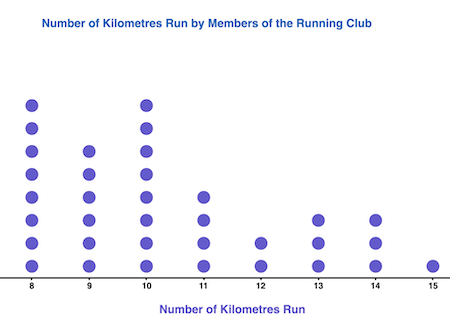
\includegraphics[width=0.75\textwidth]{dotplot.png}
    \caption{A dotplot showing the distribution of kilometers run by members of the running club.}
    \label{fig:dotplot}
\end{figure}

\emph{Dotplots} (as shown above) show each individual as a dot above their quantative data value.

When describing the shape of a dotplot (or other quantative graphs), \emph{focus on main features}: major peaks, clusters, or gaps. Especially note whether the distribution is roughly symmetric or skewed:

\begin{definition}[Symmetric, Skewed]
    A distribution is rougly \textbf{symmetric} if the right side of the graph has rougly the same shape as the left side.
    
    A distribution is \textbf{skewed to the right} if the right 'tail' has less values than the left; typically, the left has a peak whereas the right does not.
    \textbf{Left-skewed} definition are defined similarly to right-skewed distributions.
\end{definition}

For example, the distribution of the number of kilometers run is right-skewed because the right 'tail' has less values.

Graphs with a single peak are considered \emph{unimodal}, like the dotplot. Distributions with two peaks are considered \emph{bimodal}, and beyond that is considered \emph{multimodal.}

When describing a distribution of quantative data, use the acronym ROCS: \textbf{R}ange (max - min), \textbf{O}utliers (clear departures from the data), \textbf{C}enter (mean or median), and \textbf{S}hape (symmetry, skew, gaps, peaks).

Leaf plots exist. Stem represents first few digits, leaf represents final digit.

\begin{figure}[t]
    \centering
    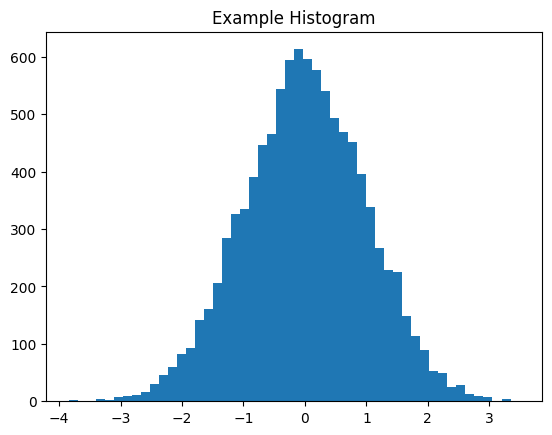
\includegraphics[width=0.75\textwidth]{histogram.png}
    \caption{An example histogram with a normal distribution.}
    \label{fig:histogram}
\end{figure}

\textbf{Histograms} are a notable way of displaying quantative data, as they avoid showing individual data points.
Histograms divide the variable into many 'bins' (bars), with the height representing the frequency. Smaller bins show more detail at the cost of a less clear pattern.

\textbf{Don't confuse histograms and bar graphs.} Histograms are used for quantative data, while bar graphs are used for qualatative data.

\textbf{Use percentages when comapring to distributions} in order to remove the effect of a larger sample.

\subsection{Describing Quantative Data with Numbers}
\begin{definition}[Mean: $\bar{x}, \mu$]
    The average of all individual data values. If there are \textit{n} observations $x_1, x_2, ..., x_n$, the sample mean is calculated by
    \[\bar{x} = \frac{\sum x_i}{n}\]
    The mean of a \textbf{sample} is referred to using $\bar{x}$, while the mean of a \textbf{population} is referred to using $\mu$.
\end{definition}

\textbf{Statistics} come from \textbf{samples} (small subset of population) and \textbf{parameters} come from \textbf{populations} (all possible samples of what's being tested).

The mean is not \textbf{resistant} as it is sensitive to strong outliers in a distribution. The median \textit{is} a resistant measure of the center of the distribution.

\begin{definition}[Median]
    The 'midpoint' of a distribution. Either the middle element ($n$ is odd) or the average of the two middle elements ($n$ is even) in a \textbf{SORTED} distribution.
\end{definition}

Using both the mean and the median, one can predict the skew of the data. If a distribution is rougly symmetric without outliers, \textbf{the mean and median will be similar}. If a distribution is strongly skewed, \textbf{the mean will be pulled in the direction of the skew}. (Mean $<$ Median for left-skewed, Mean $>$ Median for right-skewed)

The \textbf{range} (max - min) is one way to show the variability of a distribution. Note that the range is \textit{not} resistant.

\begin{definition}[Standard Deviation]
    The \textbf{standard deviation} ($s_x, \sigma$) measures the 'average' distance of the values in a distribution from the mean. Standard deviation is calculated by

    \[s_x = \sqrt{\frac{\sum{(x_i - \bar{x})^2}}{n - 1}}\]
\end{definition}

The squared stdev is known as \textbf{variance} ($s_x^2, \sigma^2$). Remember, $s_x$ refers to a sample while $\sigma$ refers to a population. Larger stdev indicates greater variation, but is not a resistant measure of variability. \textbf{Stdev measures variance around the mean; if the mean is skewed, so will stdev!}

The \textbf{Interquartile Range (IQR)} is another way to measure variance, using $IQR = Q_3 - Q_1$ where Q represents the quartiles. IQR can be thought of as the range of the 'middle half' of the distribution. \textit{IQR is a resistant measure.}

\[\textrm{Lower Outliers} < Q_1 - 1.5 \times IQR \textrm{ or High Outliers} > Q_3 + 1.5 \times IQR\]

boxplots and the five-number summary = min, Q1, median, Q3, and max exist. \textbf{Boxplots don't show gaps, clusters, or multiple peaks.}

be careful with language- 'skews' is a shape, IQR and range are single numbers (no 'in the middle of the IQR')

\newpage

\section{Modelling Distributions}
\subsection{Describing Location in a Distribution}
\begin{definition}[Percentile]
    The pth percentile of a distribution is the value with p\% of observations less than (\textit{or equal, depending on who you ask}) than it. Note that this distinction of whether or not to include "or equal" only matters for discrete variables.
\end{definition}

For example, in a class of 25 students, if a student gets a score greater than or equal to 21 other students, then they would be at the 84th percentile in the class's test score distribution ($\frac{21}{25} \approx 84\%$).
\textbf{An obervation is never "in" a percentile; an observation is AT a percentile} (percentile is just a number; like IQR and range). Also, definition, $Q_1 \approx 25$th percentile, $Q_2 \textrm{(median)} \approx 50$th percentile, and $Q_3 \approx 75$th percentile.
Percentiles can be graphically shown in a \textbf{cumulative relative frequency graph}, where the y-coordinates of points are graphed based on their percentile.

\begin{definition}[Standardized Score (z-score)]
    How many standard deviations an individual value is from the mean. For a value p, mean $\mu$, and stdev $\sigma$:
    \[z = \frac{p - \mu}{\sigma}\]
\end{definition}

z-scores provide a way to objectively compare measurements from two distributions while still considering means and variability.

\subsubsection{Transforming Data}

Effect of adding a constant a:
\begin{itemize}
    \item Adds a to measures of center and location (mean, median, quartiles, min, max)
    \item Does not change measures of variability (range, IQR, stdev)
    \item Does not change the shape of the distribution (percentile; translation along axis)
\end{itemize}

Effect of multiplying by constant b:
\begin{itemize}
    \item Multiplies measures of center and location by b (mean, median, quartiles, min, max)
    \item Multiplies measures of variability by $|b|$ (range, IQR, stdev)
    \item Does not change the \textit{overall} shape of the distribution (percentile; like squish or squash)
\end{itemize}

z-scores transform any distribution into one with mean 0 and stdev 1, but with the same original shape.

\subsection{Density Curves}
\begin{definition}[Density Curves]
    A curve that models the distribution of a quantative variable with a curve that
    \begin{itemize}
        \item Is always on (or above) the horizontal axis
        \item Has an area of exactly 1 underneath
    \end{itemize}
    The area under the curve within any interval of values estimates the proportion of all observations that fall into this interval.
\end{definition}

\textit{No set of quantative data is fully described by a density curve.} Density curves are approximations that are easy to use by smoothing out small irregularities in the data.
Similarly to finite distributions, distributions will have shapes, often with skews and peaks.

The median of the density curve splits the curve into two equal-area halves of area = 0.5.
The mean of the density curve is harder to define. For a density curve described by a function $p(x)$, the mean is given as the below.
(Intuitively, this is the idea of a 'weighted average'; weight being its relative density- $p(x)$, in this case- being extended to a continous distribution.)

\[\textrm{mean of $p(x)$} = \int_{-\infty}^{\infty}xp(x)dx\]
While the mean-median location principles still apply, they aren't too useful as it's relatively hard to locate the mean of a curve by simply looking at it.

\subsubsection{Normal Distributions}
As $\lim_{n\to\infty} n$, binomial distributions will approach a \textbf{Normal distribution} (see Chapter 6 or something), which are described using Normal curves.

\begin{definition}[Normal Curve]
    Any normal distribution is described by a symmetric, single-peaked, bell-shaped density curve. Its center is equal to the mean and the median, and the stdev represents the 'width' of the curve.
    Any normal distribution is fully described by its mean and stdev. A normal curve's mean is its peak, while the stdev are its inflection points (symmetric around the mean).

    Normal distributions with $\mu = 0$ and $\sigma = 1$ is known as a \textbf{standard Normal distribution} (which is the same as any other Normal distribution normalized into z-scores).
    \textit{Remember that mean and stdev only fully describe Normal distributions!}
\end{definition}

All normal distributions follow the \textbf{empirical rule}: 68\%, 95\%, and 99.7\% of all observations will fall within 1, 2, and 3 stdev around the mean respectively.
\verb|normalcdf(upper, lower, mean, stdev)| can be used to find the area under the normal curve (with a given mean and stdev) between upper and lower.
Similarly, \verb|invNorm(area to the left, mean, stdev)| calculates the area's percentile value given the mean and stdev.
\textbf{When using calculator functions like normalcdf, make sure to 1) label what the inputs mean and 2) answer the question asked AS A SENTENCE!}

\subsubsection{Assessing Normality}
uhh i'll do it later

\newpage

\section{Two-Variable Data}

\newpage

\section{Collecting Data}

\newpage

\section{Probability}

\newpage

\section{Random Variables and Distributions}

\newpage

\section{Sampling Distributions}

\newpage

\section{Confidence Intervals}

\newpage

\section{Significance Tests}
\textbf{Significance Tests} are like the opposite of confidence intervals. Instead of using a statistic to find a parameter, significance tests use statistics to test claims about a parameter.

\begin{definition}[Significance Test]
    A formal procedure for using observed statistics in order to decide between to competing claims (\textit{hypotheses}) about parameters.
\end{definition}

\subsection{Basics of Significance Tests}
\subsubsection{Hypotheses}
\begin{definition}[Null Hypothesis, $H_0$]
    A claim about a parameter that we weigh evidence \textbf{against} in a significance test. Usually a statement of 'no difference' (as claimed).
\end{definition}

\begin{definition}[Alternative Hypothesis, $H_a$]
    The claim that we are trying to find evidence for. Directly contradicts the null hypothesis.
\end{definition}

This "Null Hypothesis" and "Alternative Hypothesis" can be thought as trying to prove someone "guilty" or "not guilty."

For example, if a player claims they're a 80\% free throw player, the null hypothesis would be $H_0: p = 0.80$, and the alternative hypothesis would be $H_a: p < 0.80$.

The alternative hypothesis is \textbf{one-sided} because we suspect that the player makes less than 80\% of his free throws. If we believe that it's equally plausible that they make more than 80\% of their free throws, then we would use a \textbf{two-sided hypothesis}- $H_a: p \neq 0.80$.

\textbf{Hypotheses express our beliefs before looking at the data}. Molding a hypothesis around data shows nothing.

\subsubsection{P-values}
\begin{definition}[P-value]
    The probability of getting the values observed in the data under the assumption that the null hypothesis $H_0$ is true.
\end{definition}

Small P-values provide convincing evidence for the alternative hypothesis because small values suggest the observed result is unlikely to happen when the null hypothesis is true.
Similarly, large P-values provide convincing evidence for the null hypothesis because large values suggest the observed result is likely to happen due to chance if the null hypothesis is true.

In terms of probability notation: P-value = P(observed data $|$ null hypothesis is true).

For two-sided tests, we look at the distance between the null hypothesis and the observed data.
For example, if $H_0: p = 0.5$, $H_a: p \neq 0.5$ and $\hat{p} = 0.65$ (observed proportion), then the P-value = P($\hat{p} \leq 0.35$ or $\hat{p} \geq 0.6$ $|$  $p = 0.5$).
We look at $\hat{p} \leq 0.35$ because $|p - 0.35| = |p - 0.65|$.

Based on the P-value, we make a conclusion about data:
\begin{itemize}
    \item If the P-value is small (unlikely to happen by chance), then we "reject $H_0$" and conclude that there is convincing evidence for $H_a$ (in context).
    \item If the P-value is large (likely to happen by chance), then we "fail to reject $H_0$" and conclude that there is not convincing evidence for $H_a$ (in context).
\end{itemize}

How small does a P-value have to be in order to reject $H_0$? We use a given \textbf{significance value} for this boundary.

\begin{definition}[Significance Level, $\alpha$]
    The value that we use as a boundary for deciding whether a P-value is significant enough to disqualify the null hypothesis. \textit{$\alpha$ should be stated before data is produced (cherrypicking).}
    \[\textrm{P-value} < \alpha \Rightarrow \textrm{reject } H_0\ \Rightarrow \textrm{convincing evidence for $H_a$ in context}\]
    \[\textrm{P-value} > \alpha \Rightarrow \textrm{fail to reject } H_0\ \Rightarrow \textrm{not convincing evidence for $H_a$ in context}\]
\end{definition}

If P is less than the significance level, we say that the result is "statistically significant at the $\alpha = \_\_\_\_$ level."
Alternatively, "the results were significant ($P = 0.03 < \alpha = 0.05$)."
\textit{Keep in mind a P-value is more informative than a statement of significance!}

\textbf{NEVER "accept $H_0$" or conclude that $H_0$ is true!} Always use 'reject' or 'fail to reject!'

\subsubsection{Type I and Type II Errors}
When drawing a conclusion from a significance test, our conflusion may be wrong.
There are two types we can make with the conclusion process, helpfully named "Type I" and "Type II" errors. Only one type of error is possible at once.

\begin{definition}[Type I and II errors]
    A \textbf{Type I error} occurs when we reject $H_0$ when $H_0$ is true; the data gives convincing evidence that $H_a$ is true despite being false.
    
    A \textbf{Type II error} occurs when we fail to reject $H_0$ when $H_a$ is true; the data fails to give convincing evidence that $H_a$ is true despite it being true.
\end{definition}

Note $P(\textrm{Type I error}) = \alpha$.
However, significance is inversely proportional to Type II error: as significance decreases, $P(\textrm{Type II error})$ increases.

\subsubsection{Power}
\begin{definition}[Power]
    The \textbf{power} of a test is the probability that the test finds convincing evidence for $H_a$ given that the parameter is a specific value that does follow $H_a$. In other words:
    \[\textrm{power} = P(\textrm{reject $H_0$ $|$ $H_0$ is false})\]
\end{definition}

\textit{Power depends on a specific value.} For example, if the power of a test to detect p = 0.08 is 0.29 given $H_0: p = 0.10$, if the true proportion in the population is p = 0.08, there is a 0.29 probability that researchers will find convincing evidence for $H_a$.

Note Power = 1 - P(Type II Error), or written alternatively, P(Type II Error) = 1 - Power. Also note that the power of a test increases with higher sample number, higher signifiance level, further null and alternative parameter values, and 'wise choices when collecting data' (reducing variability).
\textit{Larger signifiance values reduce the chance for Type II error, but increase the chance for Type I error.}

\subsubsection{Steps for Signifiance Tests}
Overall, significance tests can be summarized in four steps:
\begin{enumerate}
    \item \textbf{STATE} the hypotheses, signifiance level, and parameters.
    \item \textbf{PLAN} the appropriate inference method and check conditions.
    \item \textbf{DO} the signifiance test (see Section 7.2): \begin{itemize}
        \item Give the sample statistic(s)
        \item Calculate the standardized test statistic
        \item Find the P-value.
    \end{itemize}
    \item \textbf{CONCLUDE} whether or not you believe in the null or alternate hypotheses, with reference to P-values, in the context of the problem. Make sure to reference the parameter, not the sample statistic!
\end{enumerate}

\subsection{Tests About a Population Proportion}

Like confidence intervals, signfiicance tests should satisfy several conditions; random sampling, no bias, 10\% if applicable ($n < 0.10N$), and large counts ($np_0 \geq 10$ and $n(1-p_0) \geq 10$).
Note that the large counts condition uses $p_0$: the number of successes and failures \textit{assuming the null hypothesis is true} are both greater than or equal to 10.

To conduct a \textbf{one-sample z test for a proportion} (CITE THIS WHEN FOLLOWING THE SIGNIFIANCE TEST STEPS) about a proportion, look at the normal distribution \textit{assuming the null hypothesis is true.}

From Section 7.2 (add ref later), $\mu_{\hat{p}} = p_0$ and $\sigma_{\hat{p}} = \sqrt{\frac{p_0(1-p_0)}{n}}$.

Using this, we standardize the statistic with respect to the null value to get the \textbf{standardized test statistic}; how many stdev units away the sample statistic is from what we would expect, assuming the null hypothesis is true.
\textbf{YOU HAVE TO PUT THE STANDARDIZED TEST STATISTIC ON THE TEST!}

\[\textrm{standardized test statistic} = z_{sts} = \frac{\hat{p} - \mu_{\hat{p}}}{\sigma_{\hat{p}}}\]

Using this, we can directly find the P-value using \verb|normalcdf| with the appropriate values:
\begin{itemize}
    \item $P(z > z_{sts})$ if $H_a : p > p_0$
    \item $P(z < z_{sts})$ if $H_a : p < p_0$
    \item $P(z > |z_{sts}|) + P(z < -|z_{sts}|)$ if $H_a : p \neq p_0$
\end{itemize}

Keep in mind that just because the P-value is low \textit{does not prove that $H_0$ is false}; sample proportions may be small due to sampling variability, or we have made a Type I error somehow. \textbf{AVOID JUMPING TO CONCLUSIONS}: just because a sample statistic looks unlikely, doesn't mean its P-value is!

It should be noted there is a link between \textit{two-sided tests} and confidence intervals: a K\% confidence interval gives an approximate set of $p_0$'s that would not be rejected by a two-sided test at the $\alpha = \frac{K}{100}$ level, with all other values being rejected.

Intuitively, if a confidence interval for p using \textit{the same} $\hat{p}$ does not include $p_0$, as the distribution (test) about $p_0$ has a similar stdev (due to the same $\alpha$) the distribution is unlikely to include the actual value of $p$.

\subsection{Tests About a Difference in Proportions}
Tests about difference in proportions work very similarly to tests about single proportions. For null hypothesis $H_0 : p_1 - p_2 = 0$, large counts can't directly be applied; we need estimate the true difference in proportions p using a weighted average of the two proportions:

\[\hat{p}_C = \frac{\textrm{number of successes in both samples combined}}{\textrm{number of individuals in both samples combined}} = \frac{n_1 \hat{p}_1 + n_2 \hat{p}_2}{n_1 + n_2}\]

We use this pooled proportion (\textit{even for non-zero differences}, although the given formulas have to be changed) because the combined proportion provides \textit{the best estimation of the true difference in proportions}.
In the one-sample z test for a proportion, we used $p_0$ because we're looking at the distribution relative to it.
For \textbf{two-sample z tests for the difference between two proportions}, we look at the distribution 'relative' to the true proportion; which our best guess is $\hat{p}_C$.

In this case, we use the combined proportion for large counts \textit{for both samples}: that is, $n_1 \hat{p}_C, n_1 (1 - \hat{p}_C), n_2 \hat{p}_C, n_2 (1 - \hat{p}_C)$ all need to be greater or equal than 10.
Using the combined proportion works for a non-zero difference in the null hypothesis, although is not strictly neccessary (large counts for each individual distribution can be used).

The standardized test statistic also uses the combined estimate (for both proportions are equal; otherwise, each individual statistic can be used):

\[z = \frac{(\hat{p}_1 - \hat{p}_2) - 0}{\sqrt{\frac{\hat{p}_C (1 - \hat{p}_C)}{n_1} + \frac{\hat{p}_C (1 - \hat{p}_C)}{n_2}}}\]

\newpage

\section{Estimating Means}

\newpage

\section{Confidence with Means}

\newpage

\section{Chi-Square Tests}

\newpage

\section{Inference for Slopes and Tables}

\[\prod_{k=1}^{4}(x^2_k+1) = \prod_{k=1}^{4}(x_k-i)(x_k+i) = \prod_{k=1}^{4}(x_k + i) \times \prod_{k=1}^4(x_k - i)\]
\[= P(i)P(-i) = (b - d + 1)^2 + (a - c)^2 = (5 - 1)^2 + 0 = \fbox{16}\]

\end{document}